\section{Zakres projektu i harmonogram}

\subsection{Zakres}

\textbf{W zakresie projektu:}
\begin{itemize}
	\item przegląd metod detekcji tekstu AI,
	\item wybór i przygotowanie zbioru danych,
	\item implementacja baseline'u (cechy statystyczne) oraz ewentualnie prostego modelu ML,
	\item ewaluacja (dokładność, precyzja/czułość w podstawowym zakresie),
	\item dokumentacja wyników i ograniczeń.
\end{itemize}

\textbf{Poza zakresem:}
\begin{itemize}
	\item detekcja w czasie rzeczywistym w produkcie komercyjnym,
	\item watermarking po stronie generatora,
	\item pełna odporność na parafrazę i ataki adversarialne,
	\item gwarancja działania dla dowolnego języka i dowolnego modelu LLM.
\end{itemize}

\subsection{Proponowane zbiory danych}

\begin{itemize}
	\item \textbf{LLM Detect AI Generated Text} (Kaggle) - gotowy zbiór do detekcji tekstu AI
	(\url{https://www.kaggle.com/datasets/sunilthite/llm-detect-ai-generated-text-dataset}).
	\item \textbf{SpeakLeash (Spichlerz)} - duży korpus tekstów polskich; źródło tekstów ludzkich do zestawu PL
	(\url{https://speakleash.org/}).
	\item \textbf{HC3 / M4} - zbiory badawcze (głównie EN): human vs ChatGPT / multi-generator.
	\item \textbf{AIDE} - eseje uczniowskie vs LLM (kontekst edukacyjny).
\end{itemize}

Na starcie planowane jest wykorzystanie zbioru z Kaggle oraz - w miarę możliwości - fragmentów SpeakLeash do eksperymentów z językiem polskim.

\subsection{Harmonogram (diagram Gantta)}

\begin{figure}[H]
\centering
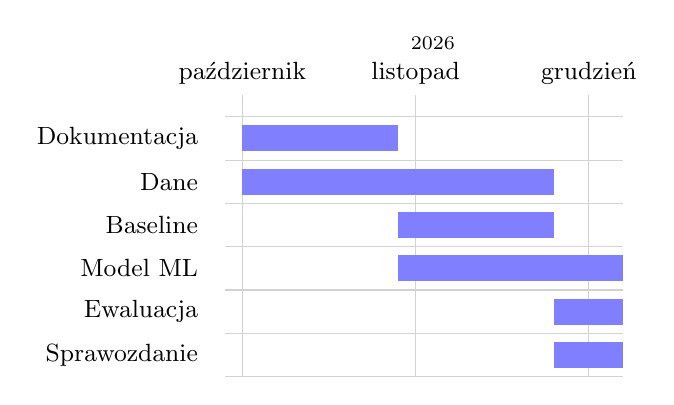
\begin{tikzpicture}[x=2.2cm,y=0.55cm]
\foreach \x/\lab in {0/październik,1/listopad,2/grudzień}
  \node[font=\small] at (\x+2.2,7) {\lab};
\node[font=\scriptsize] at (3.3,7.7) {2026};
\foreach \y in {0,...,6}
  \draw[gray!35] (2.1,\y) -- (4.4,\y);
\foreach \x in {0,...,2}
  \draw[gray!35] (\x+2.2,0) -- (\x+2.2,6.5);
\fill[blue!50] (2.2,5.2) rectangle (3.1,5.8);
\node[anchor=east,font=\small] at (2.0,5.5) {Dokumentacja};
\fill[blue!50] (2.2,4.2) rectangle (4.0,4.8);
\node[anchor=east,font=\small] at (2.0,4.5) {Dane};
\fill[blue!50] (3.1,3.2) rectangle (4.0,3.8);
\node[anchor=east,font=\small] at (2.0,3.5) {Baseline};
\fill[blue!50] (3.1,2.2) rectangle (4.4,2.8);
\node[anchor=east,font=\small] at (2.0,2.5) {Model ML};
\fill[blue!50] (4.0,1.2) rectangle (4.4,1.8);
\node[anchor=east,font=\small] at (2.0,1.5) {Ewaluacja};
\fill[blue!50] (4.0,0.2) rectangle (4.4,0.8);
\node[anchor=east,font=\small] at (2.0,0.5) {Sprawozdanie};
\end{tikzpicture}
\caption{Orientacyjny harmonogram prac (październik - grudzień 2026)}
\end{figure}
